\documentclass[aspectratio = 169]{chariteBeamer}
\usepackage[german]{babel} %% english
\usepackage[utf8]{inputenc}
\usepackage[T1]{fontenc}
\usepackage{hyperref}
\usepackage{blkarray}
\tikzset{>=latex}
\usepackage[edges]{forest}
\usetikzlibrary{positioning}
\usepackage{biostat}
\setbeamertemplate{caption}[numbered]
\let\qed\relax
\forestset{declare toks={elo}{}}
\graphicspath{{figures/}}
%% ================================================================== %% 

\author[L. Mödl, M. Becher, E. Sprünken]{Lukas Mödl, Matthias Becher, Erin Sprünken} 
\title{Tag 4 -- Control Flow} 
\date[]{Aktualisiert: \today}
\place{R-Kurs}
\email{biometrie-rkurs@charite.de}

%% ================================================================== %% 

\hyphenation{Sam-ples}
\begin{document}

\begin{frame}[plain]
    \titlepage%
\end{frame}
\frame{\tableofcontents}


\section{Programmierung I: Bedingungen}

\begin{frame}[fragile]{Konzeption if-Anweisung}
    Möchte man einen Codeblock abhängig von einem bestimmten Wert ausführen oder nicht, muss eine if-Anweisung verwendet werden. if-Anweisungen definieren einen Codeblock, der nur dann ausgeführt wird, wenn die übergebene Bedingung wahr ist. \bigskip\\
    \begin{tikzpicture}
      \node[draw, trapezium, trapezium left angle=70, trapezium right angle=-70, minimum height=0.75cm, fill=gray!50!white] (n0) {\footnotesize Code};
      \node[draw, diamond, right of=n0, node distance=4cm, fill=orange] (n1) { \footnotesize Bedingung};
      \coordinate[below of=n1, node distance=2cm] (aux1);
      \coordinate[above of=n1, node distance=2cm] (aux2);
      \node[draw, trapezium, trapezium left angle=70, trapezium right angle=-70, right of=aux2, node distance=5cm, minimum height=0.75cm,fill=pink] (n2) { \footnotesize Code};
      \node[draw, trapezium, trapezium left angle=70, trapezium right angle=-70, right of=n1, node distance=8cm, minimum height=0.75cm, fill=gray!50!white] (n3) {\footnotesize Code};
      \draw[->] (n0) to (n1);
      \draw[->] (n1.north) to (aux2) node[anchor=south]{\footnotesize Bedingung ist erfüllt} to (n2);
      \draw[->] (n2) -| (n3);
      \draw[->] (n1.south) to (aux1) node[anchor=north]{\footnotesize Bedingung ist nicht erfüllt} -| (n3);
    \end{tikzpicture}
\end{frame}

\begin{frame}[fragile]{Beispiel if-Anweisung}
  Um die Konzeption der if-Anweisung zu verstehen, soll in diesem Beispiel einer Variablen \verb+x+ der Wert \verb+3+ zugewiesen werden. Abhängig vom Wert von \verb+x+ soll dann eine Ausgabe ausgeführt werden oder nicht.\bigskip\\
      \begin{tikzpicture}
      \node[draw, trapezium, trapezium left angle=70, trapezium right angle=-70, minimum height=0.5cm, fill=gray!50!white] (n0) {\footnotesize\verb+x <- 2+};
      \node[draw, diamond, right of=n0, node distance=4cm, fill=orange] (n1) { \footnotesize \verb+x < 3+};
      \coordinate[below of=n1, node distance=2cm] (aux1);
      \coordinate[above of=n1, node distance=2cm] (aux2);
      \node[draw, trapezium, trapezium left angle=70, trapezium right angle=-70, right of=aux2, node distance=4.5cm, minimum height=0.5cm,fill=pink] (n2) {\scriptsize\verb+print("x ist kleiner als 3")+};
      \node[draw, trapezium, trapezium left angle=70, trapezium right angle=-70, right of=n1, node distance=8cm, minimum height=0.5cm, fill=gray!50!white] (n3) {\footnotesize\verb+y <- x^2+};
      \draw[->] (n0) (n0) to (n1);
      \draw[->] (n1.north) to (aux2) node[anchor=south]{\footnotesize Bedingung ist erfüllt} to (n2);
      \draw[->] (n2) -| (n3);
      \draw[->] (n1.south) to (aux1) node[anchor=north]{\footnotesize Bedingung ist nicht erfüllt} -| (n3);
    \end{tikzpicture}
\end{frame}

\begin{frame}[fragile]{Beispiel if-Anweisung}
  Um die Konzeption der if-Anweisung zu verstehen, soll in diesem Beispiel einer Variablen \verb+x+ der Wert \verb+3+ zugewiesen werden. Abhängig vom Wert von \verb+x+ soll dann eine Ausgabe ausgeführt werden oder nicht.
  \begin{center}
  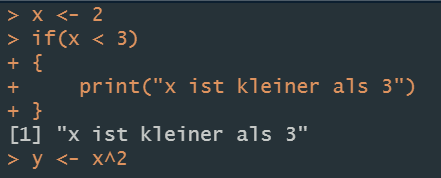
\includegraphics[]{if1.png}
  \end{center}
\end{frame}

\begin{frame}[fragile]{Konzeption if-else-Anweisung}
    Bei der if-Anweisung wird der Code, der nach der if-Anweisung steht immer ausgeführt. Das ist in einer Entweder-Oder-Situation natürlich nicht wünschenswert. Hier schafft die if-else-Anweisung Abhilfe.\bigskip\\
    \begin{tikzpicture}
      \node[draw, trapezium, trapezium left angle=70, trapezium right angle=-70, minimum height=0.75cm, fill=gray!50!white] (n0) {\footnotesize Code};
      \node[draw, diamond, right of=n0, node distance=4cm, fill=orange] (n1) { \footnotesize Bedingung};
      \coordinate[below of=n1, node distance=2cm] (aux1);
      \coordinate[above of=n1, node distance=2cm] (aux2);
      \node[draw, trapezium, trapezium left angle=70, trapezium right angle=-70, right of=aux2, node distance=4.5cm, minimum height=0.75cm,fill=pink] (n21) { \footnotesize Code};
      \node[draw, trapezium, trapezium left angle=70, trapezium right angle=-70, right of=aux1, node distance=4.5cm, minimum height=0.75cm,fill=violet!50!white] (n22) { \footnotesize Code};
      \node[draw, trapezium, trapezium left angle=70, trapezium right angle=-70, right of=n1, node distance=8cm, minimum height=0.75cm, fill=gray!50!white] (n3) {\footnotesize Code};
      \draw[->] (n0) to (n1);
      \draw[->] (n1.north) to (aux2) node[anchor=south]{\footnotesize Bedingung ist erfüllt} to (n21);
      \draw[->] (n22) -| (n3);
      \draw[->] (n21) -| (n3);
      \draw[->] (n1.south) to (aux1) node[anchor=north]{\footnotesize Bedingung ist nicht erfüllt} to (n22);
    \end{tikzpicture}
\end{frame}

\begin{frame}[fragile]{Beispiel if-else-Anweisung}
    Um die Konzeption der if-else-Anweisung zu verstehen, wird die bedingte Ausgabe des vorherigen Beispiels leicht modifiziert. \bigskip\\
    \begin{tikzpicture}
      \node[draw, trapezium, trapezium left angle=70, trapezium right angle=-70, minimum height=0.5cm, fill=gray!50!white] (n0) {\footnotesize\verb+x <- 2+};
      \node[draw, diamond, right of=n0, node distance=4cm, fill=orange] (n1) { \footnotesize \verb+x < 3+};
      \coordinate[below of=n1, node distance=2cm] (aux1);
      \coordinate[above of=n1, node distance=2cm] (aux2);
      \node[draw, trapezium, trapezium left angle=70, trapezium right angle=-70, right of=aux2, node distance=4.5cm, minimum height=0.5cm,fill=pink] (n21) { \scriptsize \verb+print("x ist kleiner als 3")+};
      \node[draw, trapezium, trapezium left angle=70, trapezium right angle=-70, right of=aux1, node distance=4.5cm, minimum height=0.5cm,fill=violet!50!white] (n22) { \scriptsize \verb+print("x ist nicht kleiner als 3")+};
      \node[draw, trapezium, trapezium left angle=70, trapezium right angle=-70, right of=n1, node distance=8cm, minimum height=0.5cm, fill=gray!50!white] (n3) {\footnotesize \verb+y <- x^2+};
      \draw[->] (n0) to (n1);
      \draw[->] (n1.north) to (aux2) node[anchor=south]{\footnotesize Bedingung ist erfüllt} to (n21);
      \draw[->] (n22) -| (n3);
      \draw[->] (n21) -| (n3);
      \draw[->] (n1.south) to (aux1) node[anchor=north]{\footnotesize Bedingung ist nicht erfüllt} to (n22);
    \end{tikzpicture}
\end{frame}

\begin{frame}[fragile]{Beispiel if-else-Anweisung}
    Um die Konzeption der if-else-Anweisung zu verstehen, wird die bedingte Ausgabe des vorherigen Beispiels leicht modifiziert. \bigskip\\
  \begin{center}
  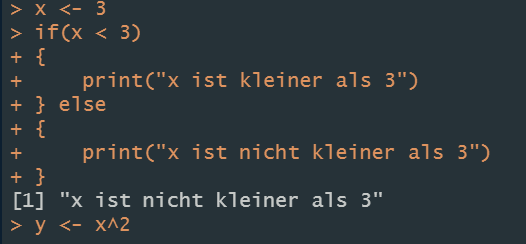
\includegraphics[]{if2.png}
  \end{center}
\end{frame}

\begin{frame}[fragile]{Anmerkungen zur if-else-Anweisung}
  \begin{itemize}
    \item Das Setzen der geschweiften Klammern \verb+{+ und \verb+}+ ist essenziell!
    \item Als Bedingungen sind nur logische Ausdrücke zugelassen 
    \item Manchmal sind verschachtelte if-else-Anweisungen nötig
    \item Für bessere Lesbarkeit des Codes empfiehlt es sich, Codeblöcke mit Tab einzurücken
  \end{itemize}
\end{frame}

\section{Programmierung II: Schleifen}

\begin{frame}[fragile]{Konzeption for-Schleife}
    Eine beiden wesentlichen Schleifen in \textsf R ist die for-Schleife. for-Schleifen führen einen Codeblock so oft aus, wie eine Laufvariable Werte in einer Indexmenge (einem Vektor oder einer Liste) annehmen kann. Die for-Schleife wird mit dem Schlüsselwort \verb+for()+ gefolgt von einem Codeblock in geschweiften Klammern eingeleitet. In den runden Klammern wird die Laufvariable über die Indexmenge initialisiert. \bigskip\\
    \begin{tikzpicture}
      \node[draw, trapezium, trapezium left angle=70, trapezium right angle=-70, minimum height=0.75cm, fill=gray!50!white] (n0) {\footnotesize Code};
      \node[draw, trapezium, trapezium left angle=70, trapezium right angle=-70, right of=n0, node distance=12cm, minimum height=0.75cm, fill=gray!50!white] (nx) {\footnotesize Code};
      \coordinate[below of=n0, node distance=2cm] (aux1);
      \coordinate[below of=nx, node distance=2cm] (aux2);
      \node[draw, circle, right of=n0, node distance=6cm, fill=blue!50!white] (n1) { \footnotesize for-\newline\footnotesize Schleife};
      \node[rectangle, draw, right of=aux1, node distance=2cm,fill=blue!50!white] (n2) {\footnotesize Laufvariable wird initialisiert};
      \node[draw, trapezium, trapezium left angle=70, trapezium right angle=-70, below of=n1, node distance=2cm, minimum height=0.75cm,fill=violet!50!white] (n3) { \footnotesize Code};
      \node[rectangle, draw, below of=n3, node distance=1cm,fill=blue!50!white] (n4) {\footnotesize Laufvariable wird inkrementiert};
      \node[rectangle, draw, right of=n3, node distance=4cm,fill=blue!50!white] (n5) {\footnotesize Laufvariable in Indexmenge};
      \draw[->] (n0) to (n1);
      %\draw[->] (n1) to (nx);
      \coordinate[below of=n1, node distance=1.25cm] (aux3);
      \draw[->] (n1.south) -- (aux3) -| (n2.north);
      \draw[->] (n2) to (n3);
      \draw[->] (n5) to node[anchor=north]{\footnotesize ja} (n3);
      \draw[<-] (n5) |- (n4);
      \draw[->] (n3) to (n4);
      \draw[->] (n5.east) -| node[anchor=south west]{\footnotesize nein} (nx.south);
    \end{tikzpicture}
\end{frame}

\begin{frame}[fragile]{Beispiel for-Schleife}
  Die Funktionsweise der for-Schleife soll an diesem Beispiel verdeutlicht werden. Hier entspricht \verb+I+ der Indexmenge und \verb+i+ Bezeichnet die Laufvariable.\bigskip\\
    \begin{tikzpicture}
      \node[draw, trapezium, trapezium left angle=70, trapezium right angle=-70, minimum height=0.5cm, fill=gray!50!white] (n0) {\footnotesize \verb+I = c(1,2,3,4,5)+};
      \node[draw, trapezium, trapezium left angle=70, trapezium right angle=-70, right of=n0, node distance=12cm, minimum height=0.5cm, fill=gray!50!white] (nx) {\footnotesize\verb+print("Ende")+};
      \coordinate[below of=n0, node distance=2cm] (aux1);
      \coordinate[below of=nx, node distance=2cm] (aux2);
      \node[draw, circle, right of=n0, node distance=6cm, fill=blue!50!white] (n1) { \footnotesize for-\newline\footnotesize Schleife};
      \node[rectangle, draw, right of=aux1, node distance=2cm,fill=blue!50!white] (n2) {\footnotesize\verb+i <- 1+};
      \node[draw, trapezium, trapezium left angle=70, trapezium right angle=-70, below of=n1, node distance=2cm, minimum height=0.5cm,fill=violet!50!white] (n3) { \footnotesize \verb+print(i)+};
      \node[rectangle, draw, below of=n3, node distance=1cm,fill=blue!50!white] (n4) {\footnotesize \verb$i <- i + 1$};
      \node[rectangle, draw, right of=n3, node distance=4cm,fill=blue!50!white] (n5) {\footnotesize \verb+i <= 5+};
      \draw[->] (n0) to (n1);
      %\draw[->] (n1) to (nx);
      \coordinate[below of=n1, node distance=1.25cm] (aux3);
      \draw[->] (n1.south) -- (aux3) -| (n2.north);
      \draw[->] (n2) to (n3);
      \draw[<-] (n3) to node[anchor=north]{\footnotesize ja} (n5);
      \draw[<-] (n5) |- (n4);
      \draw[->] (n3) to (n4);
      \draw[->] (n5.east) -| node[anchor=south west]{\footnotesize nein} (nx.south);
    \end{tikzpicture}
\end{frame}

\begin{frame}[fragile]{Beispiel for-Schleife}
  Die Funktionsweise der for-Schleife soll an diesem Beispiel verdeutlicht werden. Hier entspricht \verb+I+ der Indexmenge und \verb+i+ Bezeichnet die Laufvariable.\bigskip\\
  \begin{centering}
  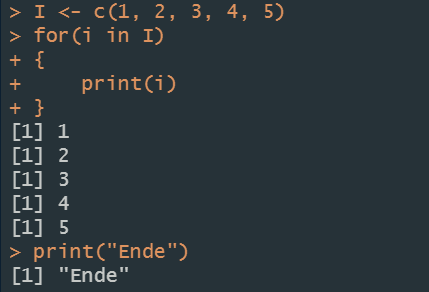
\includegraphics[]{for1.png}
  \end{centering}
\end{frame}

\subsection*{while-Schleife}

\begin{frame}[fragile]{Konzeption while-Schleife}
Die andere wesentliche Schleife ist die while-Schleife. Im Gegensatz zur for-Schleife wird hier ein Codeblock so lange ausgeführt, wie eine gegebene Bedingung erfüllt ist. Die while-Schleife wird mit dem Schlüsselwort \verb+while()+ gefolgt von einem Codeblock in geschweiften Klammern eingeleitet. Innerhalb der runden Klammern wird die Bedingung übergeben. \bigskip\\
   \begin{tikzpicture}
      \node[draw, trapezium, trapezium left angle=70, trapezium right angle=-70, minimum height=0.75cm, fill=gray!50!white] (n0) {\footnotesize Code};
      \node[draw, trapezium, trapezium left angle=70, trapezium right angle=-70, right of=n0, node distance=12cm, minimum height=0.75cm, fill=gray!50!white] (nx) {\footnotesize Code};
      \coordinate[below of=n0, node distance=2cm] (aux1);
      \coordinate[below of=nx, node distance=2cm] (aux2);
      \node[draw, circle, right of=n0, node distance=6cm, fill=blue!50!white] (n1) { \footnotesize while-\newline\footnotesize Schleife};
      \node[draw, trapezium, trapezium left angle=70, trapezium right angle=-70, below of=n1, node distance=2cm, minimum height=0.75cm,fill=violet!50!white] (n3) { \footnotesize Code};
      \node[rectangle, draw, right of=n3, node distance=4cm, fill=blue!50!white] (n5) {\footnotesize Bedingung ist erfüllt};
      \draw[->] (n0) to (n1);
      \coordinate[below of=n1, node distance=1.35cm] (aux4);
      \coordinate[below of=n3, node distance=1cm] (aux5);
      \draw[->] (n1.south) -- (aux4) -| (n5.north);
      \draw[->] (n3) to (n5);
      \draw[->] (n5) |- node[anchor=west]{\footnotesize ja} (aux5) -| (n3);
      \draw[->] (n5.east) -| node[anchor=south west]{\footnotesize nein} (nx.south);
    \end{tikzpicture}
\end{frame}

\begin{frame}[fragile]{Beispiel while-Schleife}
  Das folgende Beispiel erklärt die Funktionsweise der while-Schleife. Die Bedingung hier ist \verb+x >= 0+.\bigskip\\
     \begin{tikzpicture}
      \node[draw, trapezium, trapezium left angle=70, trapezium right angle=-70, minimum height=0.5cm, fill=gray!50!white] (n0) {\footnotesize \verb+x <- 10+};
      \node[draw, trapezium, trapezium left angle=70, trapezium right angle=-70, right of=n0, node distance=12cm, minimum height=0.5cm, fill=gray!50!white] (nx) {\footnotesize \verb+print("Ende")+};
      \coordinate[below of=n0, node distance=2cm] (aux1);
      \coordinate[below of=nx, node distance=2cm] (aux2);
      \node[draw, circle, right of=n0, node distance=6cm, fill=blue!50!white] (n1) { \footnotesize while-\newline\footnotesize Schleife};
      \node[draw, trapezium, trapezium left angle=70, trapezium right angle=-70, below of=n1, node distance=2cm, minimum height=0.5cm,fill=violet!50!white,text width=1.75cm] (n3) { \footnotesize \verb+print(x)+\\\footnotesize \verb+x <- x - 1+};
      \node[rectangle, draw, right of=n3, node distance=4cm, fill=blue!50!white] (n5) {\footnotesize \verb+x >= 0+};
      \draw[->] (n0) to (n1);
      \coordinate[below of=n1, node distance=1.35cm] (aux4);
      \coordinate[below of=n3, node distance=1cm] (aux5);
      \draw[->] (n1.south) -- (aux4) -| (n5.north);
      \draw[->] (n3) to (n5);
      \draw[->] (n5) |- node[anchor=west]{\footnotesize ja} (aux5) -| (n3);
      \draw[->] (n5.east) -| node[anchor=south west]{\footnotesize nein} (nx.south);
    \end{tikzpicture}
\end{frame}

\begin{frame}[fragile]{Beispiel for-Schleife}
  Das folgende Beispiel erklärt die Funktionsweise der while-Schleife. Die Bedingung hier ist \verb+x >= 0+.\bigskip\\
  \begin{centering}
  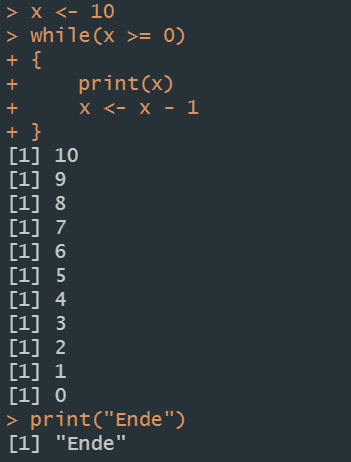
\includegraphics[]{while1.png}
  \end{centering}
\end{frame}

\subsection*{Anmerkungen zu for- und while-Schleifen}

\begin{frame}[fragile]{Anmerkungen zu for- und while-Schleifen}
  \begin{itemize}
    \item Das Setzen das geschweiften Klammern \verb+{+ und \verb+}+ ist essenziell!
    \item Vorsicht vor unendlichen Schleifen!
    \item Jede for-Schleife kann auch als while-Schleife programmiert werde und umgekehrt
    \item Mit \verb+break+ kann eine Schleife beendet werden
    \item Mit \verb+next+ kann eine Iteration übersprungen werden, ohne dass die Schleife beendet wird
    \item Die \verb+apply+-Familie bietet oft eine praktische Alternative zu Schleifen
    \end{itemize}
\end{frame}

\subsection*{Die Apply-Familie}

\begin{frame}[fragile]{Apply-Familie}
	Die Apply-Familie ist eine Reihe von Funktion in R, die es uns erlaubt eine Funktion auf mehrere verschiedenen Inputs nacheinander anzuwenden. Zum Beispiel auf alle Zeilen oder Spalten einer Matrix oder alle Elemente einer Liste. Die verschiedenen Apply-Funktionen sind:  
	\begin{itemize}
		\item \verb+apply()+
		\item \verb+lapply()+
		\item \verb+sapply()+
		\item \verb+tapply()+
	\end{itemize}
\end{frame}

\begin{frame}[fragile]{apply()}
	Mit apply() können wir Funktionen auf alle Zeilen oder Spalten eines Data Frames oder einer Matrix anwenden um zum Beispiel alle Spaltensummen zu berechnen. Die Grundform der Funktion ist:
	\begin{itemize}
		\item \verb+apply(data, margin, function)+
	\end{itemize}
	Zum Beispiel:
	\begin{columns}[T]
		\begin{column}{0.5\textwidth}
			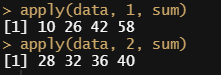
\includegraphics{Apply}
		\end{column}
		\begin{column}{0.4\textwidth}
			\[
			\renewcommand\BAextrarowheight{2pt}
			\begin{blockarray}{*{5}{c}}
				\begin{block}{[*{4}{c}]{c}}
				    1 &2 &3 &4&\textcolor{red}{10}\\
				    5 &6 &7 &8&\textcolor{red}{26}\\
				    9 &10 &11 &12&\textcolor{red}{42}\\
				    13 &14 &15 &16&\textcolor{red}{58}\\
				\end{block}
				\textcolor{red}{28} & \textcolor{red}{32} & \textcolor{red}{36} & \textcolor{red}{40}
			\end{blockarray}
			\]
		\end{column}
	\end{columns}
	
\end{frame}

\begin{frame}[fragile]{lapply()}
	lapply() führt eine Funktion auf jedes Element eines Data Frames, einer Matrix, eines Vektors oder einer Liste aus. Das "l" in lapply() steht dabei für "list" und bezieht sich darauf, dass lapply() immer eine Liste zurück gibt.
	\begin{itemize}
		\item \verb+lapply(object, function)+
	\end{itemize}
	Zum Beispiel:\\
	\begin{center}
		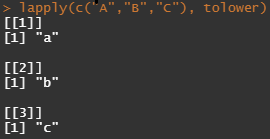
\includegraphics{lapply}
	\end{center}
	
	
\end{frame}

\begin{frame}[fragile]{sapply()}
	sapply() macht im Grunde das gleiche wie lapply(). Der Unterschied ist, dass sapply() einen Vektor oder eine Matrix zurück gibt, anstatt eine Liste:
	\begin{itemize}
		\item \verb+sapply(object, function)+
	\end{itemize}
	Zum Beispiel:\\
	\begin{center}
		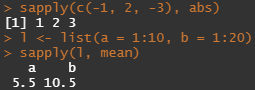
\includegraphics{sapply}
	\end{center}
\end{frame}

\begin{frame}[fragile]{tapply()}
	tapply() erlaubt es uns auf Grundlage von factor levels Gruppenzusammenfassungen zu erstellen:
	\begin{itemize}
		\item \verb+tapply(object, index, function)+
	\end{itemize}
	Zum Beispiel:\\
	\begin{center}
		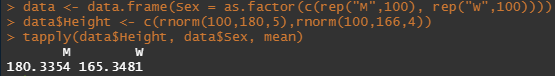
\includegraphics{tapply}
	\end{center}
\end{frame}

\section{Eigene Funktionen}

\begin{frame}[fragile]{Konzeption eigener Funktionen}
    Bisher haben wir nur vordefinierte Funktionen wie beispielsweise \verb+t.test+ verwendet. \textsf R erlaubt es aber auch, eigene Funktionen zu schreiben.\bigskip\\
    Funktionen sind ein eigener Datentyp, der mit dem Schlüsselwort \verb+function()+ intialisiert werden muss, gefolgt von einem Codeblock in geschweiften Klammern. Innerhalb der runden Klammern können freie Variablen definiert werden, die von der zu definierenden Funktion als Argumente interpretiert werden. 
\end{frame}

\begin{frame}[fragile]{Beispiel für eine Funktion mit einem Argument}
  Bei der Funktion $f(x) = x^2$ entspricht $x$ einer freien Variablen. Die Funktion wird wie folgt in \textsf R implementiert:\bigskip\\
  \begin{centering}
    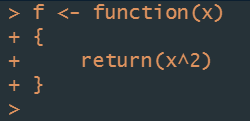
\includegraphics[]{func1.png}
  \end{centering}
\end{frame}

\begin{frame}[fragile]{Anmerkungen zur Definition eigener Funktionen}
  \begin{itemize}
    \item Das Setzen das geschweiften Klammern \verb+{+ und \verb+}+ ist essenziell!
    \item Werden Argumente spezifiziert, müssen die bei jedem Aufruf der Funktion übergeben werden\\Eine Ausnahme bilden freie Variablen, die innerhalb der runden Klammern des Schlüsselworts \verb+function()+ mittels \verb+=+ initialisiert wurden
    \item Sollen mehrere freie Variablen übergeben werden, müssen diese mit Komma getrennt werden 
    \item Sofern möglich \textsf R vektorisiert Funktionen automatisch, d.h. wird ein Vektor oder eine Matrix als Argument übergeben, wird die Funktion auf jedes Element einzeln angewendet
    \item Soll eine Funktion keinen Wert zurückgeben, kann auf \verb+return+ verzichtet werden
  \end{itemize}
\end{frame}



\end{document}
